\documentclass{standalone}
\usepackage{tikz}
\usetikzlibrary{calc}
\usetikzlibrary{automata, positioning, arrows}
\tikzstyle{inarrow}=[->, >=stealth, shorten >=.03cm,line width=0.5]
\begin{document}
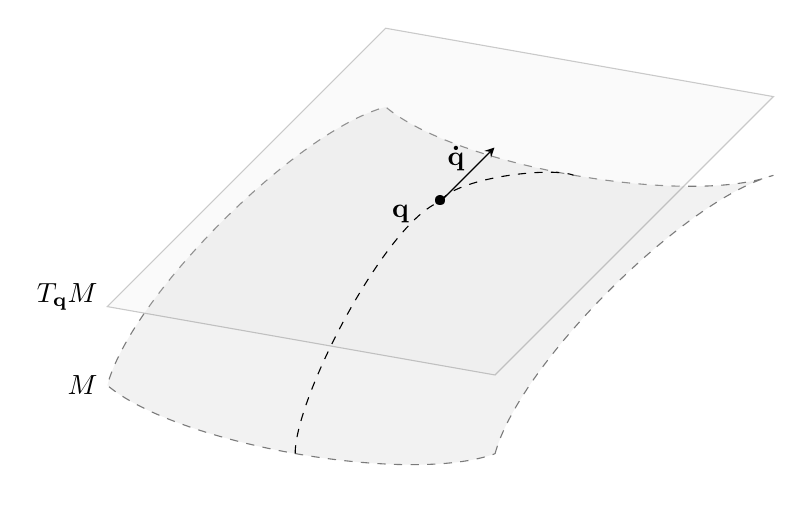
\begin{tikzpicture}[x={({cos(-10)*1cm},{sin(-10)*1cm})},y={({cos(45)*1cm},{sin(45)*1cm})},z={(0,1cm)}]
  \draw[dashed, fill=gray!20, opacity=0.5, looseness=.6] 
    (2.5,-2.5,-1)
    to[bend left] coordinate (mk) (2.5,2.5,-1)
    to[bend left] coordinate (mp) (-2.5,2.5,-1) 
    to[bend right] coordinate (mq) (-2.5,-2.5,-1) coordinate (labelM)
    to[bend right] coordinate (mm) (2.5,-2.5,-1)
    -- cycle;
  \node[left] at (labelM) {$M$};
  \draw[fill=gray!20, opacity=0.2] 
    (2.5,-2.5,0)
    -- (2.5,2.5,0) 
    -- (-2.5,2.5,0)
    -- (-2.5,-2.5,0) coordinate (labelTM) 
    -- cycle;
  \node[above right, label=left:$T_\mathbf{q}M$] at (labelTM) {};
  \draw[dashed,looseness=.5] (mm) to[in=200, out=90] (0,0,0) to[out=60, in=160] (mp);
  \node (q) at (0,0,0) {\textbullet};
    \node at (-0.3,-0.3,0) {$\mathbf{q}$};
  \draw[inarrow] (0,0,0) -- (0,1,0);
    \node at (-0.3,0.7,0) {$\mathbf{\dot{q}}$};
  
\end{tikzpicture}
\end{document}